\documentclass[tikz,border=10pt]{standalone}
\begin{document}
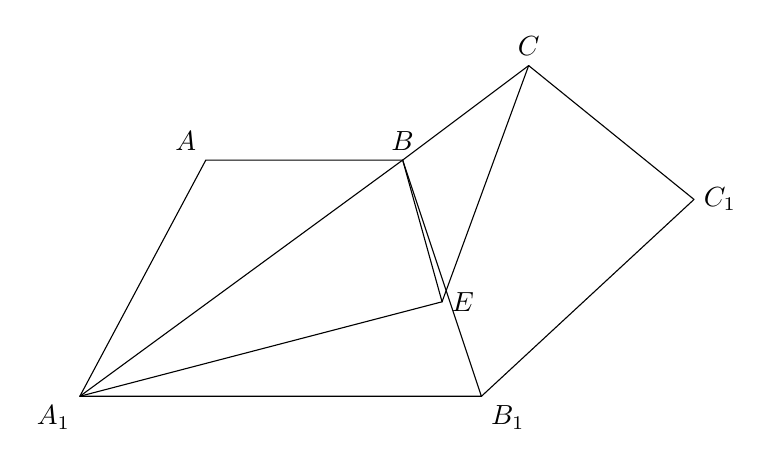
\begin{tikzpicture}[line join=round, line cap=round, scale=1]

\coordinate (A1) at (0,0);
\coordinate (A)  at (1.6,3.0);
\coordinate (B)  at (4.1,3.0);
\coordinate (B1) at (5.1,0.0);
\coordinate (E)  at (4.6,1.2);
\coordinate (C)  at (5.7,4.2);
\coordinate (C1) at (7.8,2.5);

\draw (A1) -- (A) -- (B) -- (B1) -- (A1);
\draw (A1) -- (B);
\draw (A1) -- (E);
\draw (B) -- (E);
\draw (E) -- (C);
\draw (B) -- (C);
\draw (C) -- (C1) -- (B1);

\node[above left] at (A) {$A$};
\node[above] at (B) {$B$};
\node[below left] at (A1) {$A_1$};
\node[below right] at (B1) {$B_1$};
\node[right] at (E) {$E$};
\node[above] at (C) {$C$};
\node[right] at (C1) {$C_1$};

\end{tikzpicture}
\end{document}
